\documentclass{beamer}
\usepackage[orientation=portrait,size=a0,scale=1.4,debug]{beamerposter}
\mode<presentation>{\usetheme{ZH}}
\usepackage{chemformula}
\usepackage[utf8]{inputenc}
\usepackage[english]{babel} % required for rendering German special characters
\usepackage{siunitx} %pretty measurement unit rendering
\usepackage{hyperref} %enable hyperlink for urls
\usepackage{ragged2e}
\usepackage[font=scriptsize,justification=justified]{caption}
\usepackage{array,booktabs,tabularx}

\newcolumntype{Z}{>{\centering\arraybackslash}X} % centered tabularx columns
%\sisetup{per=frac,fraction=sfrac}

\title{\huge Zero-shot Crate Digging $\rightarrow$ DJ Tool retrieval using Speech Activity, Music Structure and CLAP embeddings}
\author{Iroro Orife}
\institute[ETH]{Independent}
\date{\today}

% edit this depending on how tall your header is. We should make this scaling automatic :-/
\newlength{\columnheight}
\setlength{\columnheight}{104cm}

\begin{document}
\begin{frame}
\begin{columns}
	\begin{column}{.43\textwidth}
		\begin{beamercolorbox}[center]{postercolumn}
			\begin{minipage}{.98\textwidth}  % tweaks the width, makes a new \textwidth
				\parbox[t][\columnheight]{\textwidth}{ % must be some better way to set the the height, width and textwidth simultaneously
				
				
				     % TOP LEFT SECTION
					\begin{myblock}{What are DJ Tools?}
					In genres like Hip-Hop, RnB, Reggae, Dancehall and every Electronic/Dance/Club style, DJ tools are a special set of audio files of short, simplified musical phrases retrieved, curated from existing music, or composted specifically to heighten the DJ's musical performance and creative mixing choices.
						
						\vspace{0.7em}

						\begin{itemize}
							\item Acapella loops, vocal chants, spoken word, one shot vocal samples
							\item Purely instrumental (no drums) piano, guitar, strings, horns 
							\item Drum loops, solo percussion, drum breaks
							\item Sound effects: risers, sweeps, sirens, vinyl fx, 
							\item Scratch and Battle loops

						\end{itemize}
						\vspace{0.7em}

						\begin{figure}
							\begin{minipage}{0.43\textwidth}
								\centering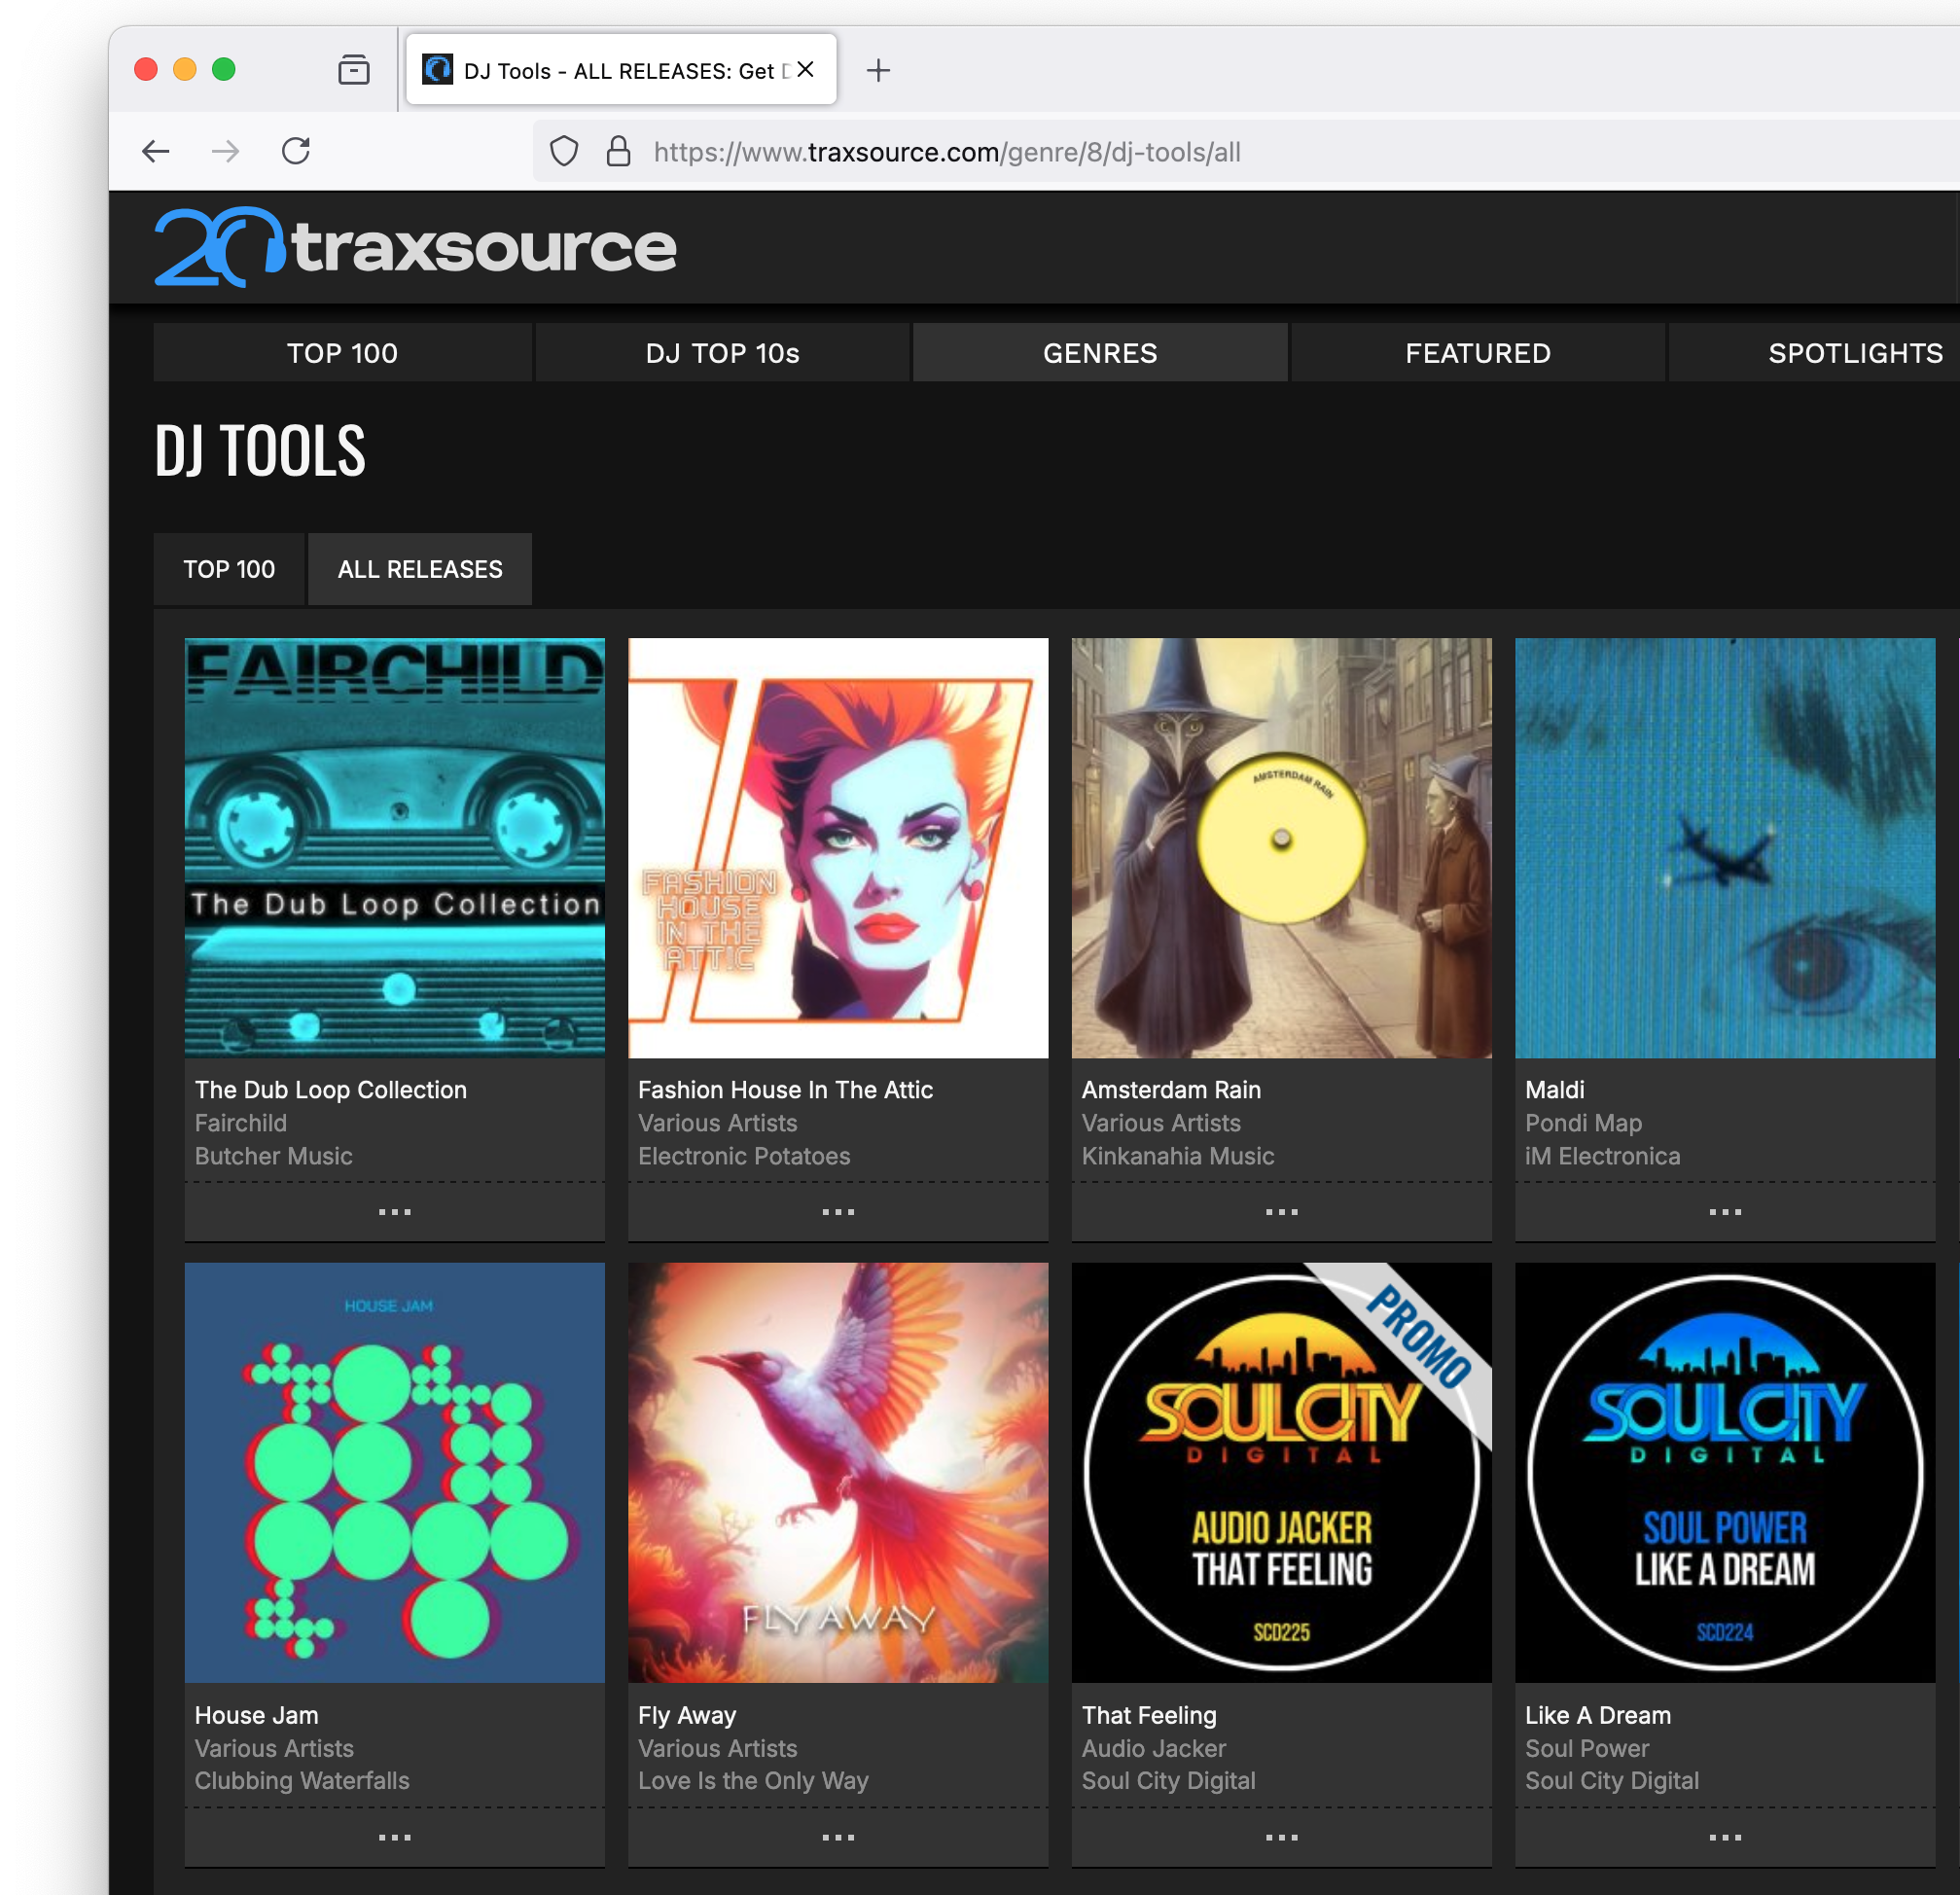
\includegraphics[width=0.8\textwidth]{img/traxsource_djtools.png}
								\caption{Traxsource DJ Tools shop}
							\end{minipage}
						\end{figure}


			            \begin{figure}
			              \begin{minipage}{0.43\textwidth}
			                \centering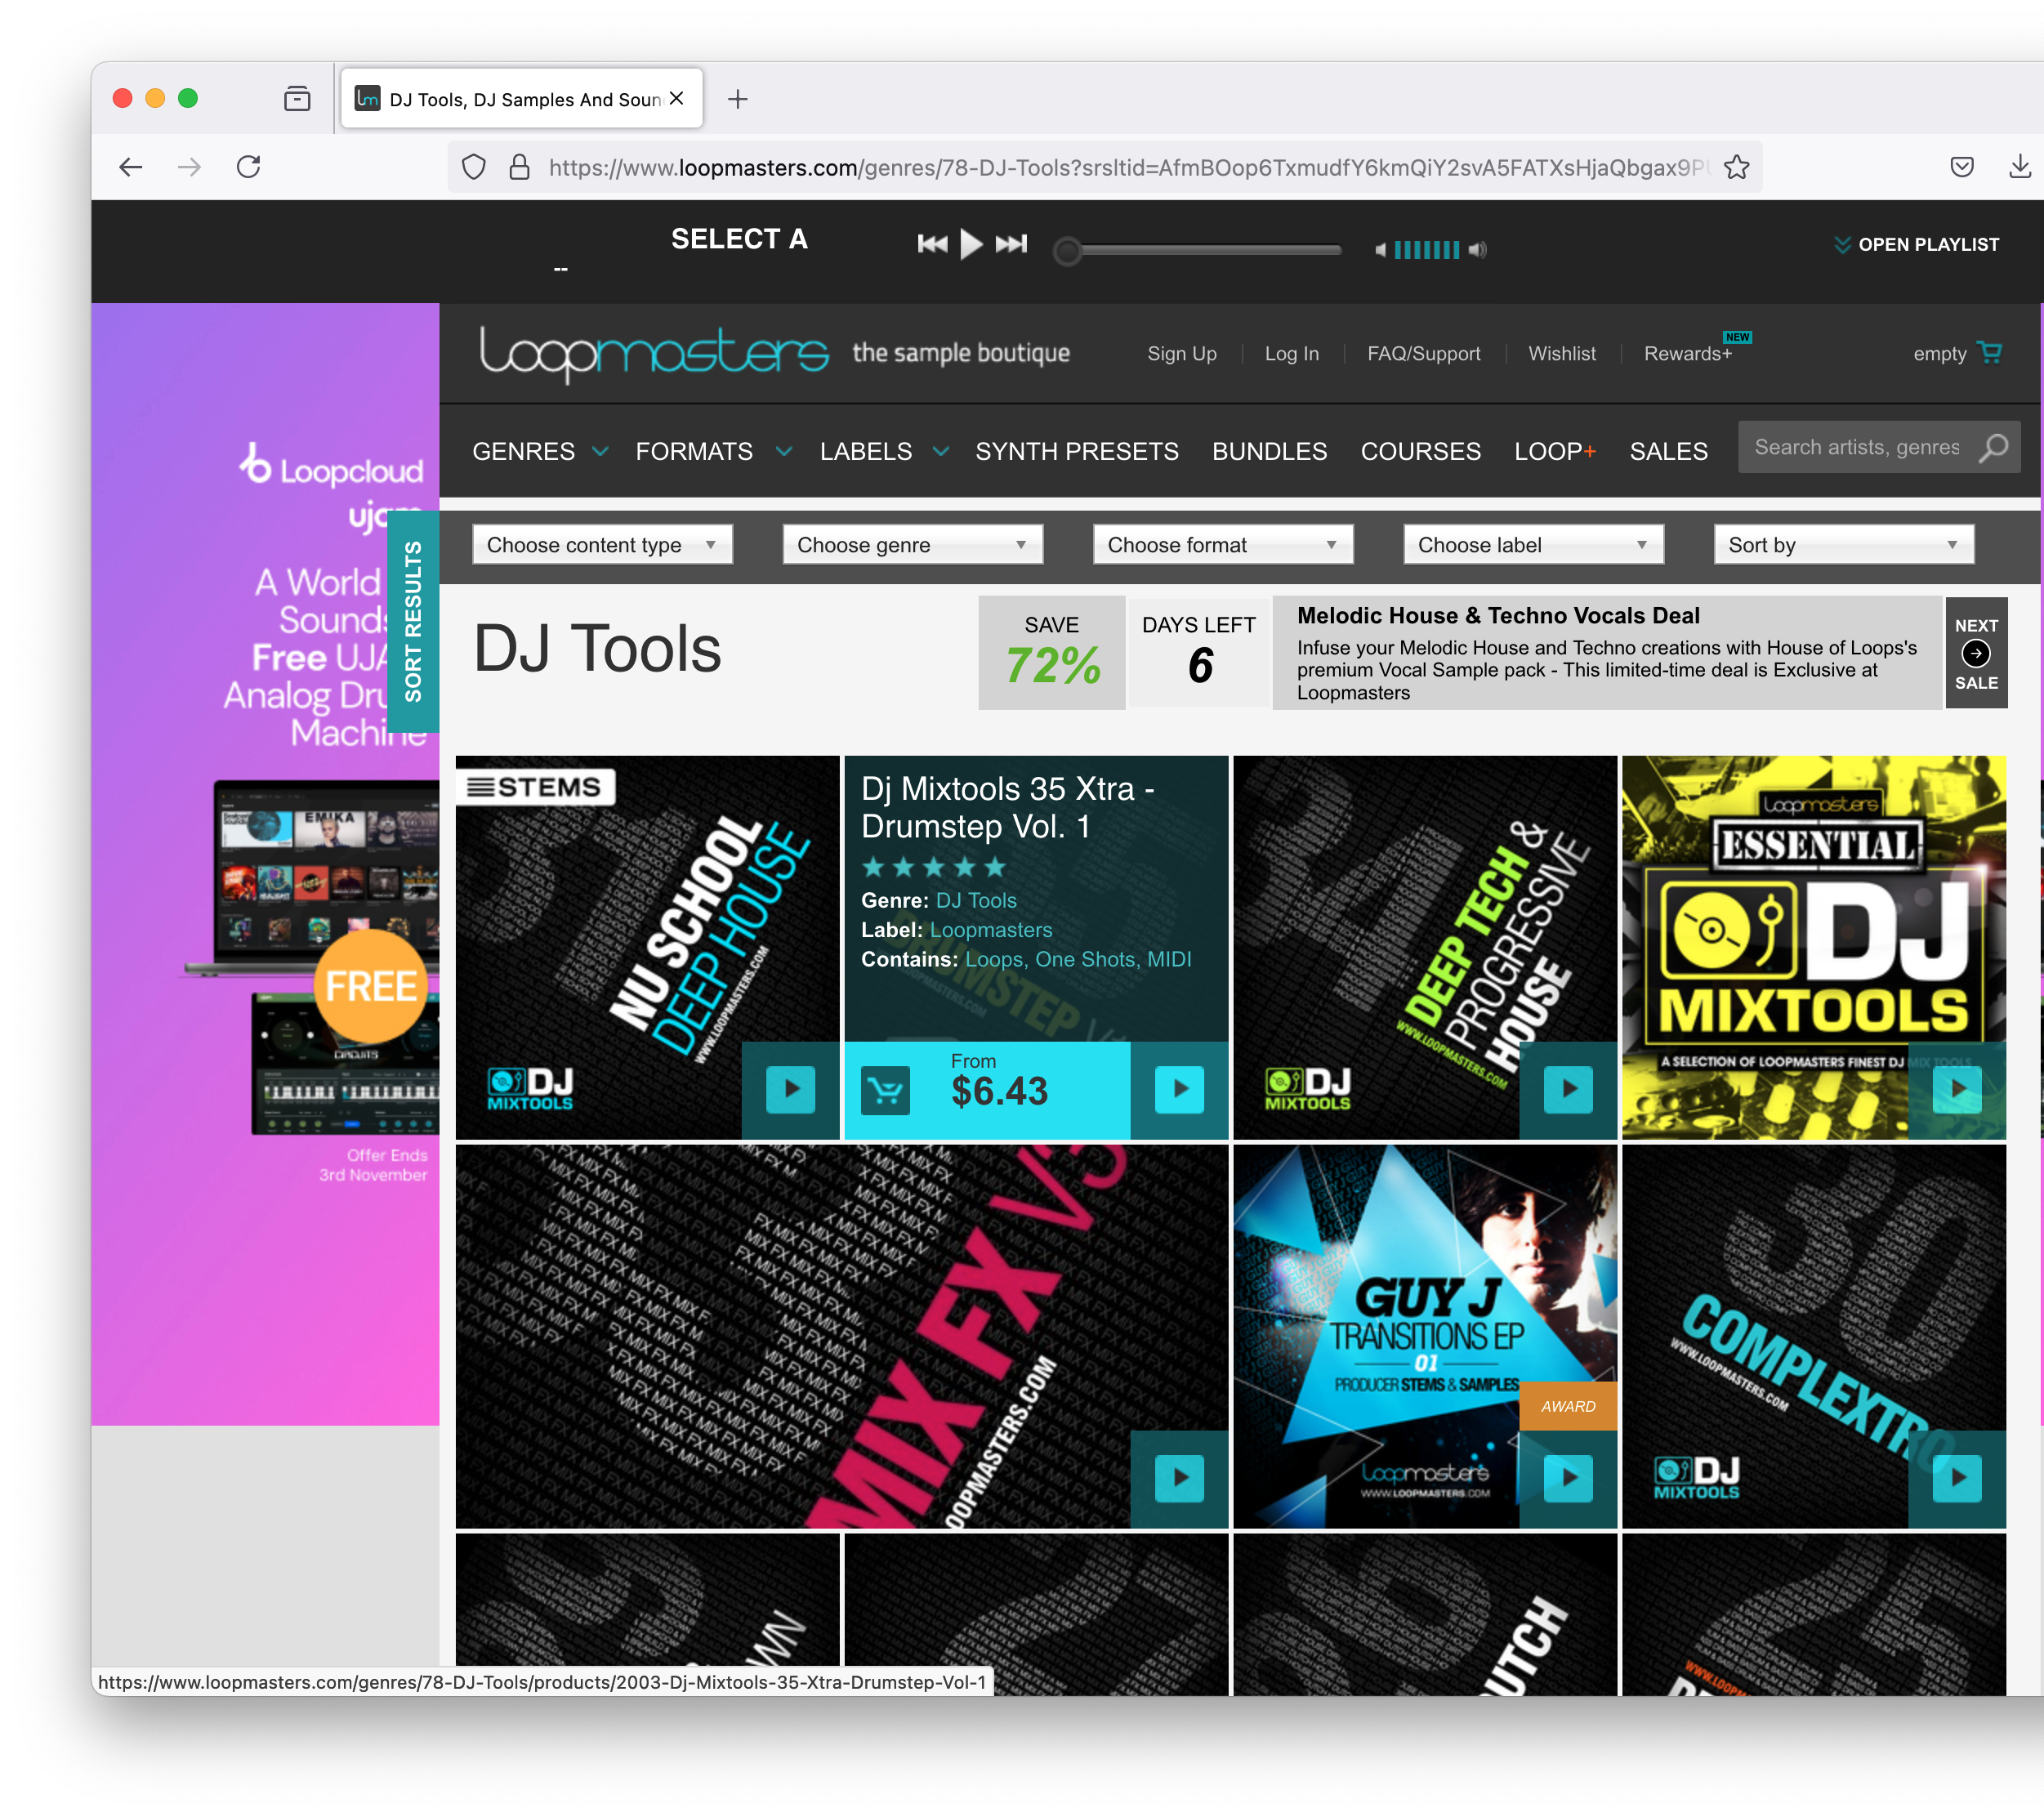
\includegraphics[width=0.85\textwidth]{img/loopmasters_djtools.png}
			                \caption{Loopmasters online shop. Note the specification of Loops, One-shots}
			              \end{minipage}
			              \hspace{1em}
			              \begin{minipage}{0.45\textwidth}
			                \centering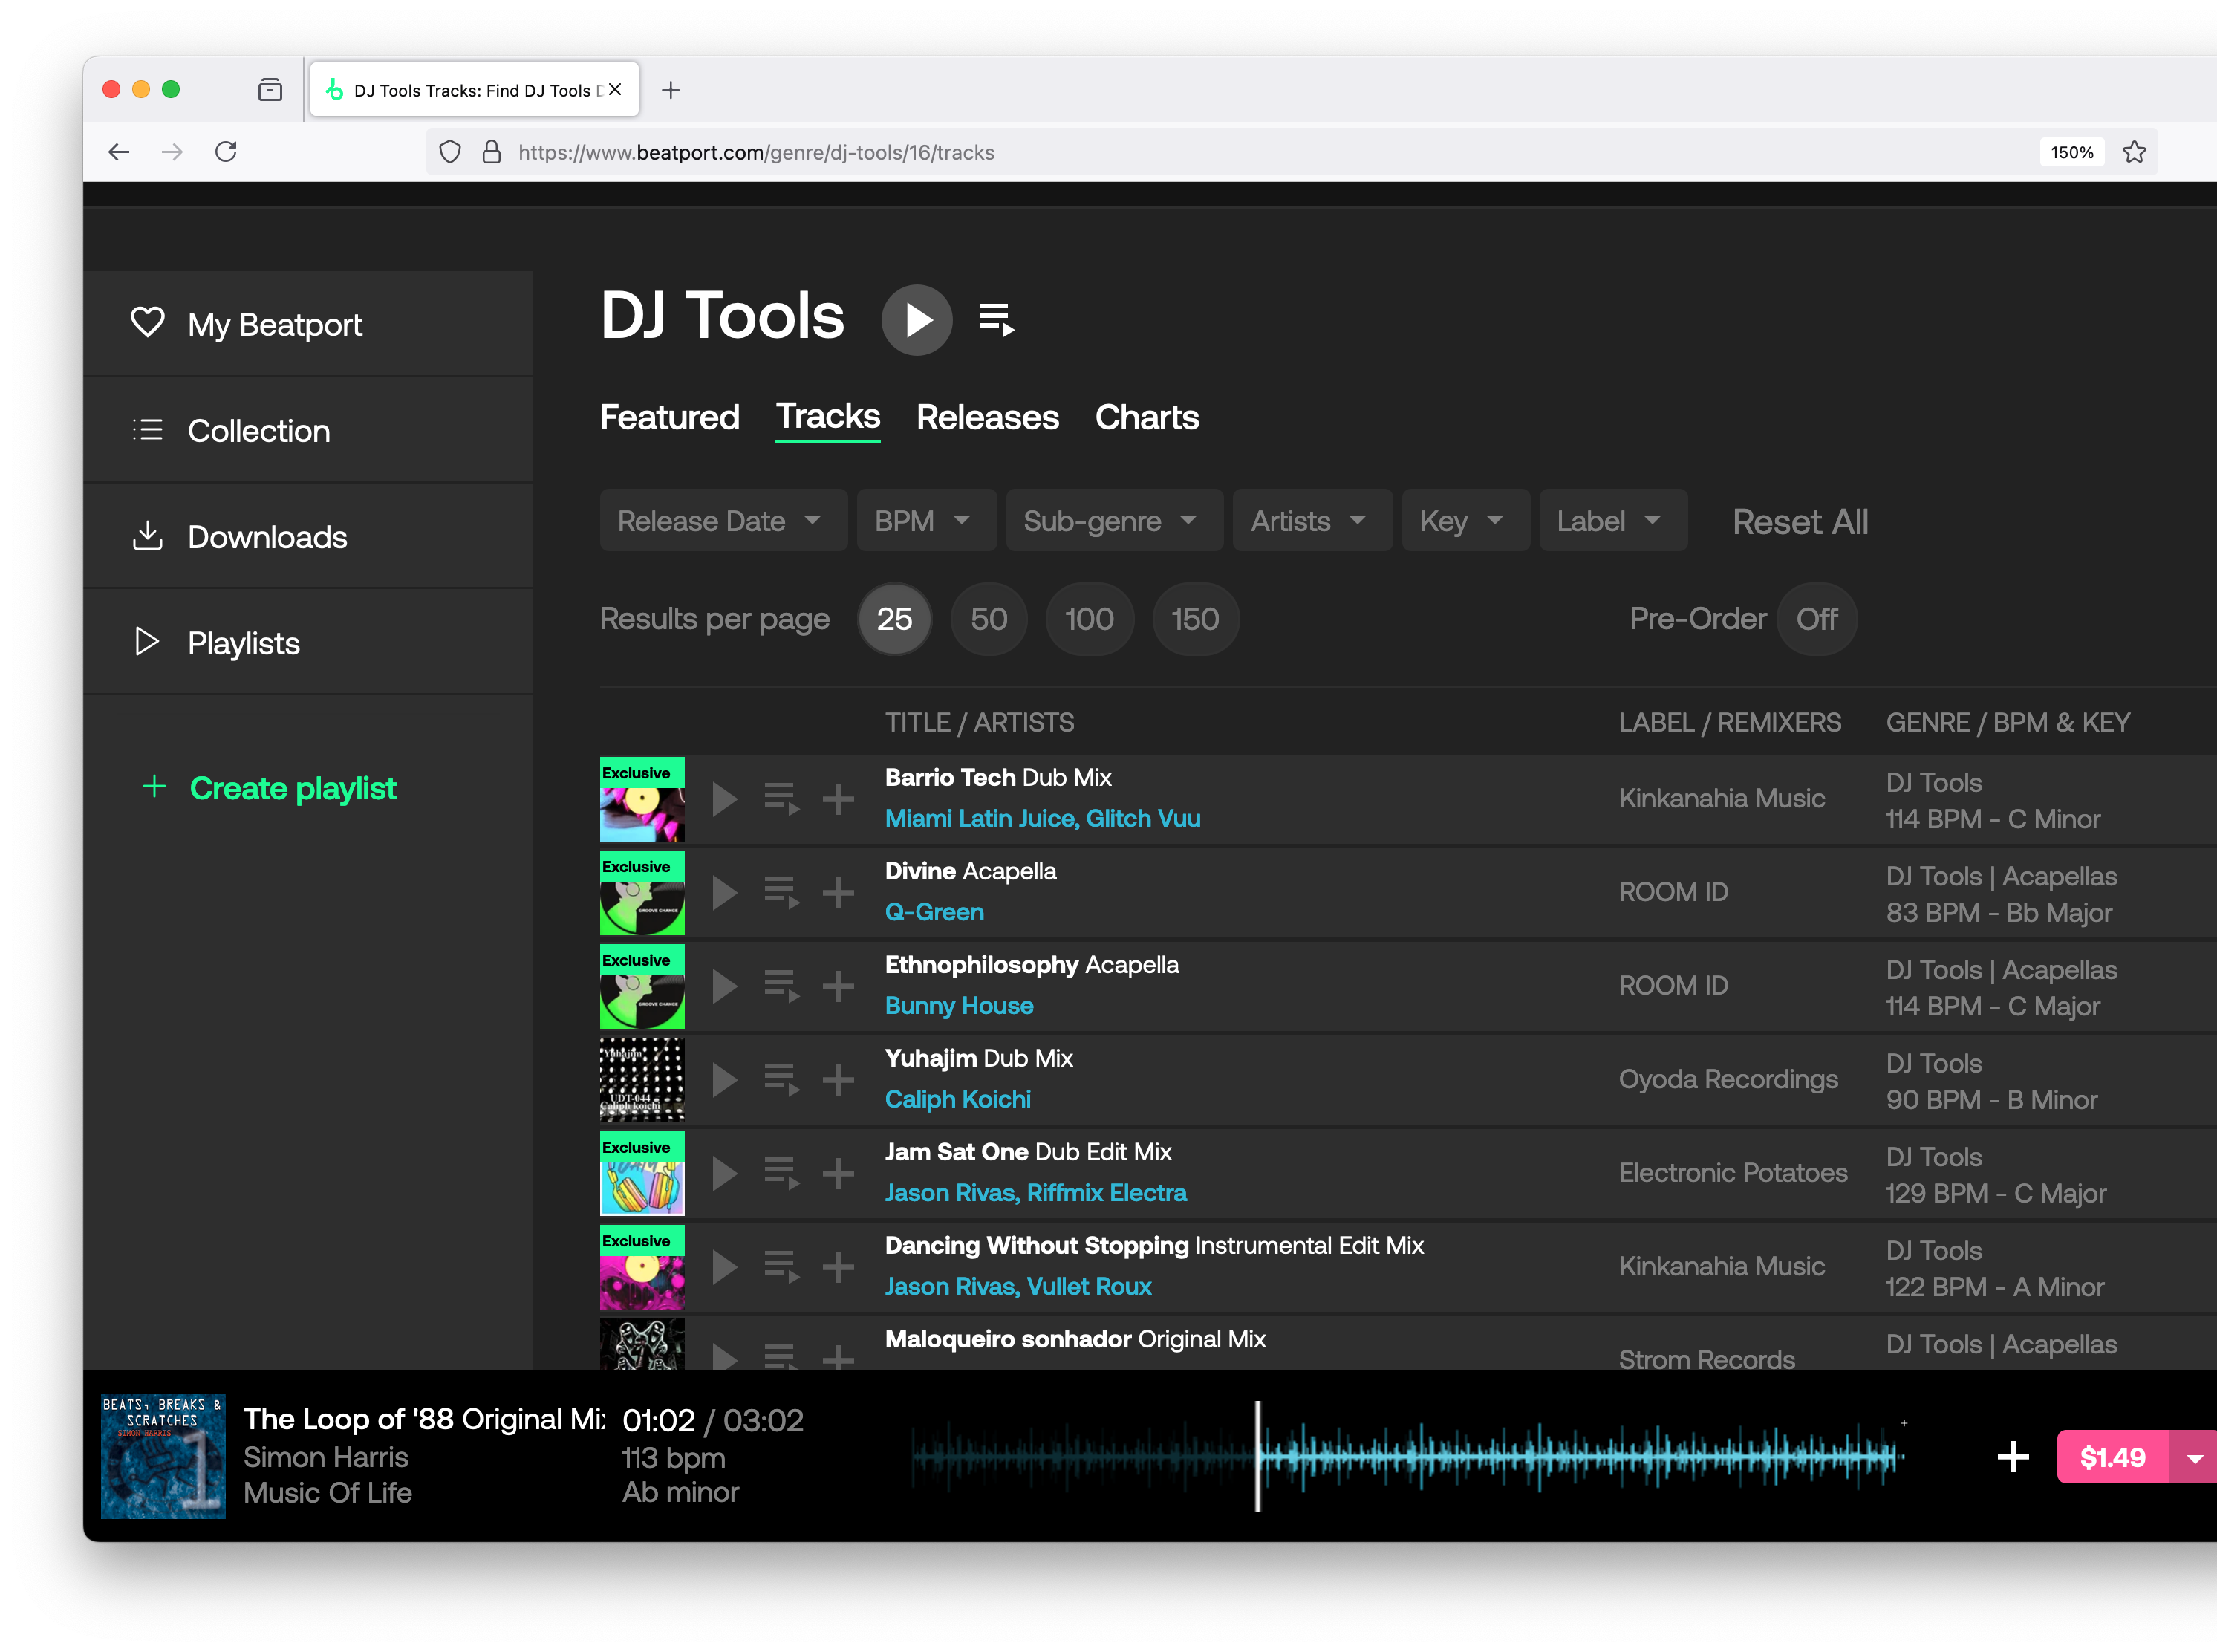
\includegraphics[width=1\textwidth]{img/beatport_djtools.png}
			                \caption{Beatport DJ Tools selection. Note the designated Genre, Key and BPM metadata}
			              \end{minipage}
			            \end{figure}
					\end{myblock}\vfill
					
%					BOTTOM LEFT SECTION
					\begin{myblock}{Speech Activity \& Music Structure Analysis}
					
					The DJ-tool classification system and its dependencies are fully open-source software (OSS) written in Python.\footnote{https://github.com/ruohoruotsi/djtool-crate-digging} Firstly, we run MSAF\footnote{https://github.com/urinieto/msaf} and SMAD\footnote{https://github.com/biboamy/TVSM-dataset/tree/master} to generate raw activities and structural boundaries, saved as CSV files\cite{Hung2022, nieto2016systematic}. Next, these are post-processed to yield lists of segment time ranges. Figure \ref{fig:msafsmadplot} shows the relationship between the boundaries and the speech activity for one song. For zero-shot classification, we utilize the LAION version of CLAP\footnote{https://huggingface.co/laion/clap-htsat-unfused} hosted on Huggingface\cite{elizalde2022claplearningaudioconcepts, WuClap2023}. Finally, we manually create a list of descriptive text strings for each class, as listed in Table \ref{tab:djtool_texts}.
					
					\vspace{0.7em}
	
			\begin{figure}
			 \centerline{
			 	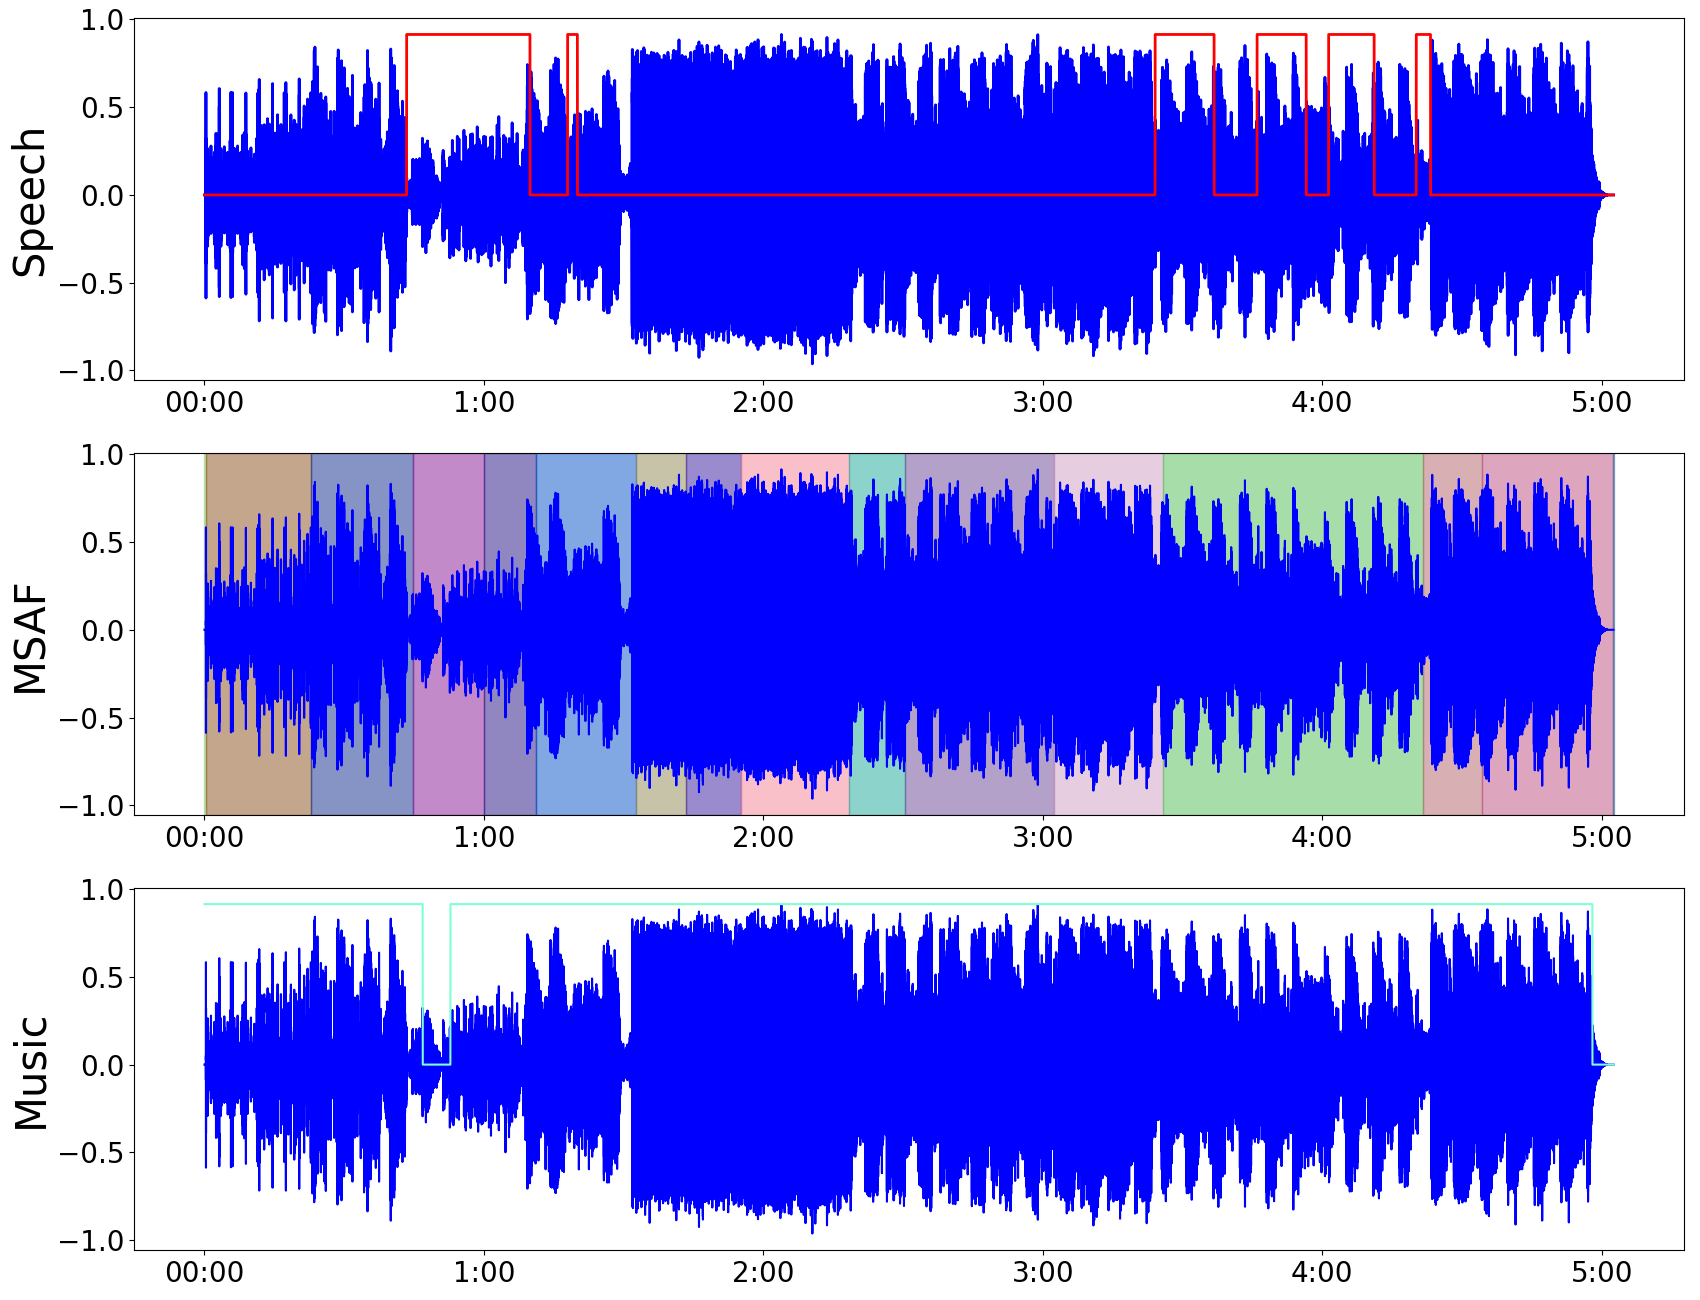
\includegraphics[alt={SMAD \& MSAF Analysis signals}, width=0.6\columnwidth]{img/smad_msaf.png}}
			 \caption{A 5 minute Ragga Jungle song overlaid with detected speech, \\ music activity and music-structural boundaries}
			 \label{fig:msafsmadplot}
			\end{figure}

%
			\begin{table}
			 \begin{center}
			 \begin{tabular}{ll}
			  \midrule
			  \textbf{DJ Tool class} & \textbf{Example text description} \\
			  \midrule
				Acapella loops & ``expressively sung vocal tracks''  \\
				Sound effects &  ``siren, riser sound effects, whoosh''\\
				Drums breaks  & ``drum beat, drum solo, breakbeat''  \\
				Melodic hooks & ``strings, solo guitar, piano melodies''  \\
				DJ Drops & ``a high energy, massive EDM drop''  \\
				Battle tracks & ``vinyl scratch loop, turnatablism''   \\
			 \end{tabular}
			\end{center}
			 \caption{In practise, text descriptions are more tortuous}
			 \label{tab:djtool_texts}
			\end{table}


					\end{myblock}\vfill
		}\end{minipage}\end{beamercolorbox}
	\end{column}
	
	
	
	% TOP RIGHT SECTION
	\begin{column}{.57\textwidth}
		\begin{beamercolorbox}[center]{postercolumn}
			\begin{minipage}{.98\textwidth} % tweaks the width, makes a new \textwidth
				\parbox[t][\columnheight]{\textwidth}{ % must be some better way to set the the height, width and textwidth simultaneously
					\begin{myblock}{What is Zero-shot Audio Classification?}
						
						\vspace{0.2em}
						\begin{figure}
							\begin{minipage}{.94\textwidth}
								\centering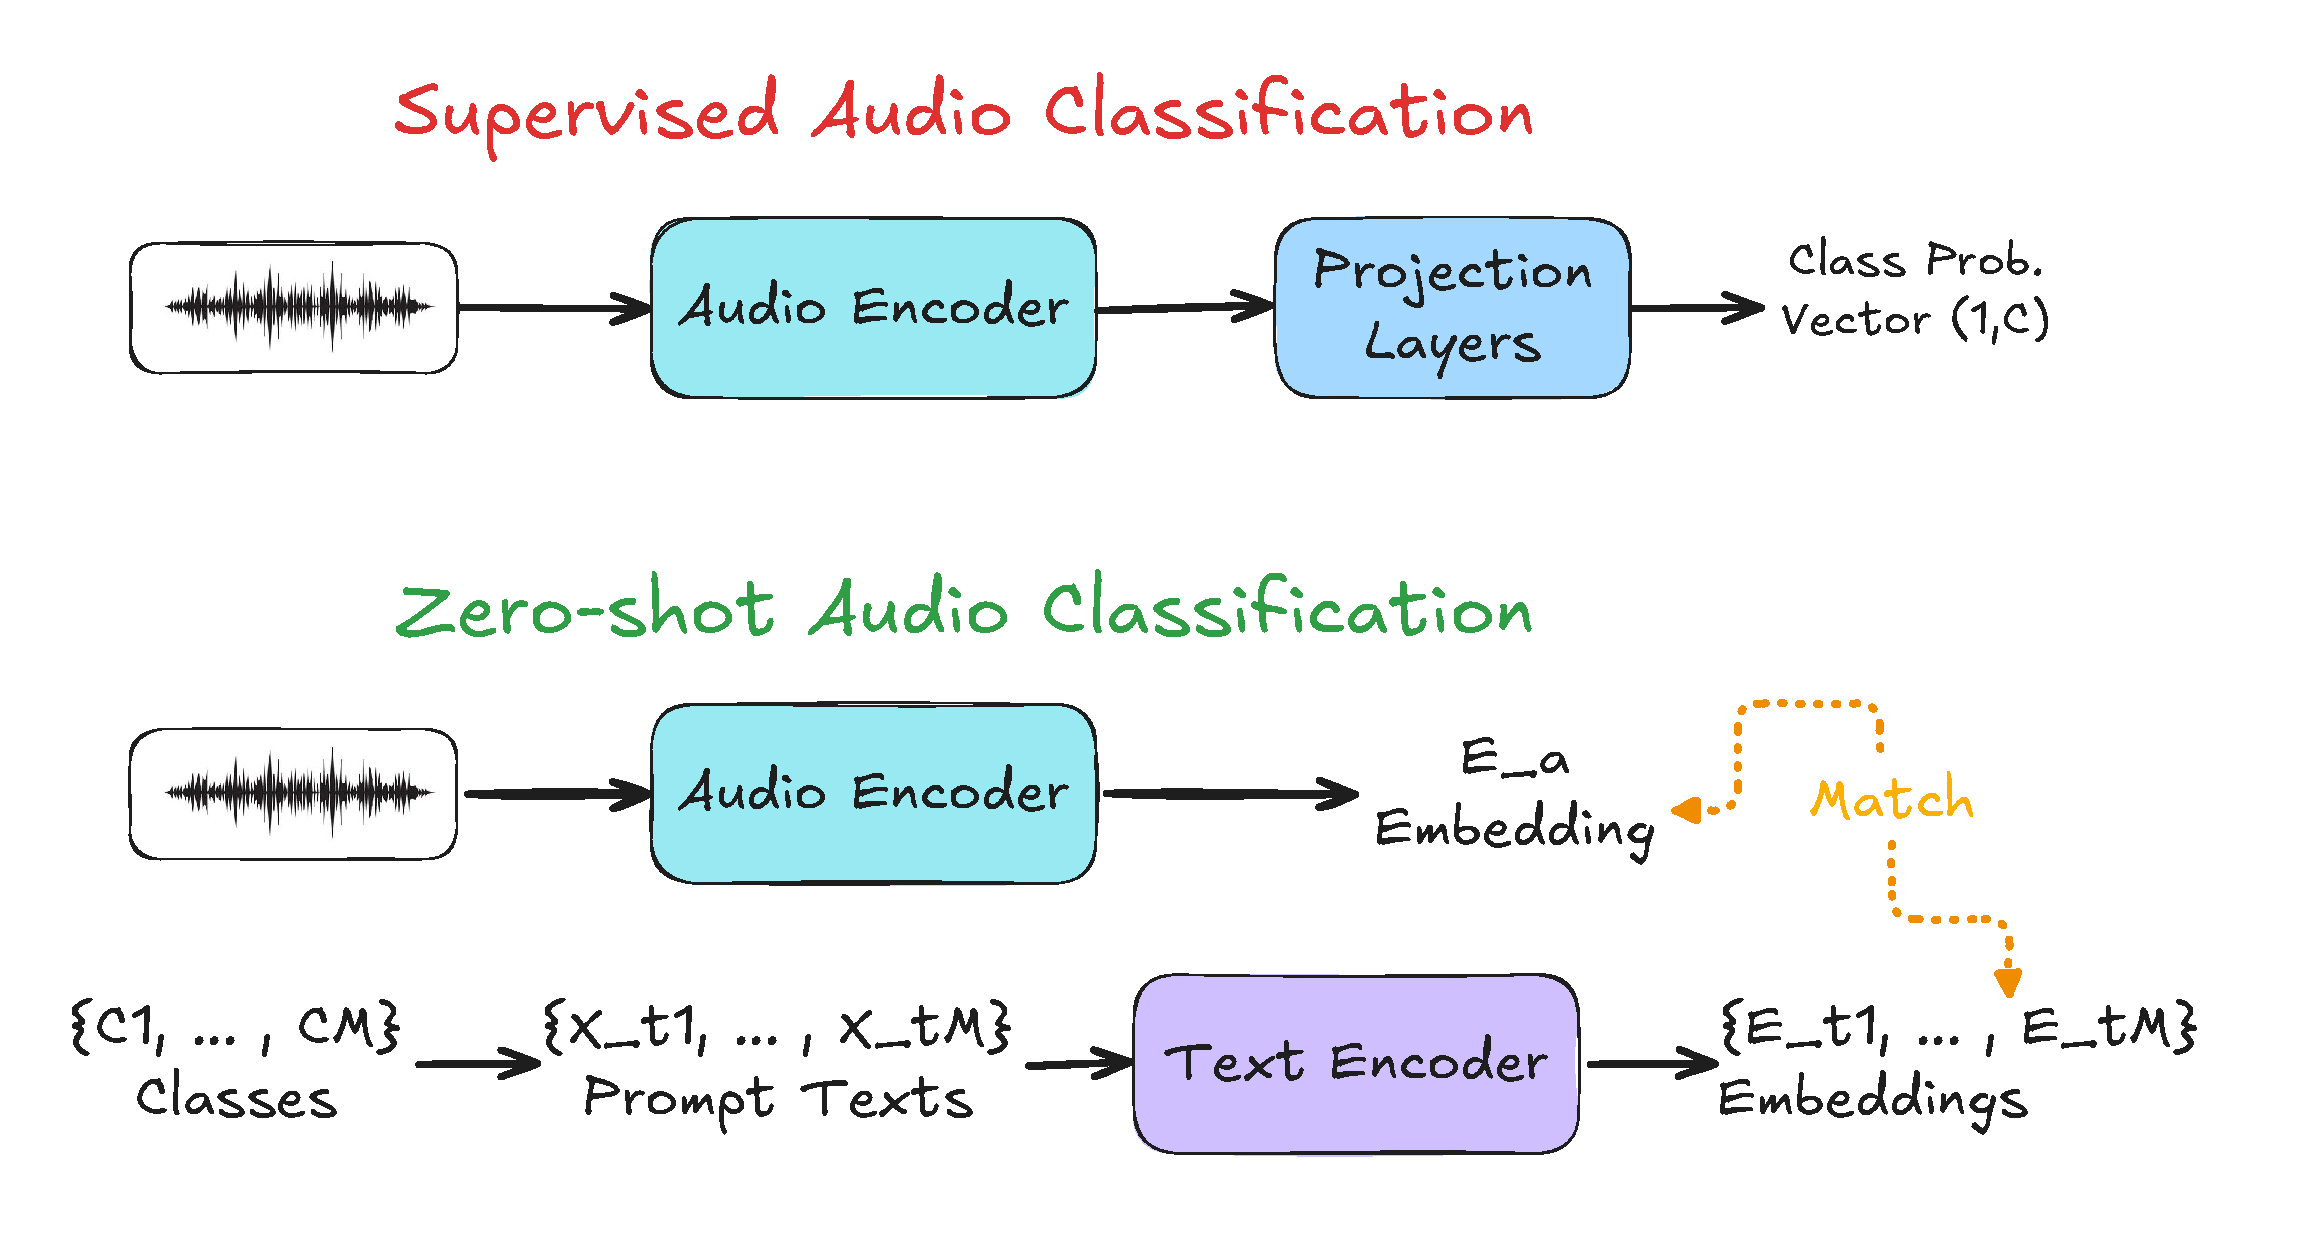
\includegraphics[width=\textwidth]{img/CLAP-ISMIR_lbd.pdf}
								\caption{}
							\end{minipage}
						\end{figure}
						\vspace{0.4em}
						
						\vspace{0.1em}

						\vspace{1em}
						

					\end{myblock}\vfill
					
					
			     % BOTTOM RIGHT SECTION
					\begin{myblock}{Crate digging: A short history of DJ tool}
					
					Before the advent of online shops trading sonic tools, DJs and producers were known to spend time in record shops crate-digging, or hunting for rare, vintage, or otherwise obscure vinyl with interesting breaks, melodic hooks, drops, intros/outros, or B-side acapellas. Practise time was devoted to studying the structure of music, identifying suitable mix points, curating tools and experimenting with different creative interpolations between two mixable songs. Then while playing live, tools are triggered or looped from Sampler modules or ``Remix Decks'' connected to the DJ mixing board.



%						\begin{figure}
%							\begin{minipage}{0.85\textwidth}
%								\centering\includegraphics[width=0.75\textwidth]{img/fail.png}
%								\caption{Contrast for all stimulation train parameter estimates for the pre-drug-administration session (red) and the acute fluoxetine administration session (green). Note the considerably different scales.}
%								\label{fig:fail}
%							\end{minipage}
%						\end{figure}
					\end{myblock}\vfill
					
					
					% BOTTOM RIGHT SECTION
					\begin{myblock}{Making music with the system}
						Preliminary results from the comparison of the first two measurement sessions (as seen in figure~\ref{fig:tt}) indicate that the uncorrected response to optogenetic stimulation across all trains (depicted individually in figure~\ref{fig:stim}) is stronger and more widespread immediately after acute fluoxetine administration than in the drug-naive mouse.
						
					\end{myblock}\vfill
					
					
					
					\begin{myblock}{References}
						\footnotesize
						\bibliographystyle{abbrv}
						\bibliography{./bib}
					\end{myblock}\vfill
		}\end{minipage}\end{beamercolorbox}
	\end{column}
\end{columns}
\end{frame}
\end{document}
